Multicore processors are ubiquitous, from phones, desktops, to high-end servers.
False sharing occurs when multiple tasks, running on different cores with private L1 caches, access logically independent words in the same cache line. When a thread modifies data of a cache line, the underlying cache coherence protocol (inside hardware) silently invalidates the duplicates of this cache line on other cores. Unnecessary synchronizations caused by false sharing can dramatically degrade the performance of parallel software by up to an order of magnitude ~\cite{falseshare:effect}. A simple example shown in Figure~\ref{fig:penalty} also exemplifies this catastrophic performance effect of false sharing. The hardware trend, including adding more cores into the same machine, introducing the Non-Uniform-Memory-Access (NUMA) architecture, or increasing the size of a cache line, will further degrade the performance of false sharing problems, making the task of detecting even more urgent. 

\begin{figure*}[htbp]
\centering
\subfigure[Parallel Programs]{%
   \label{fig:penaltycode}
   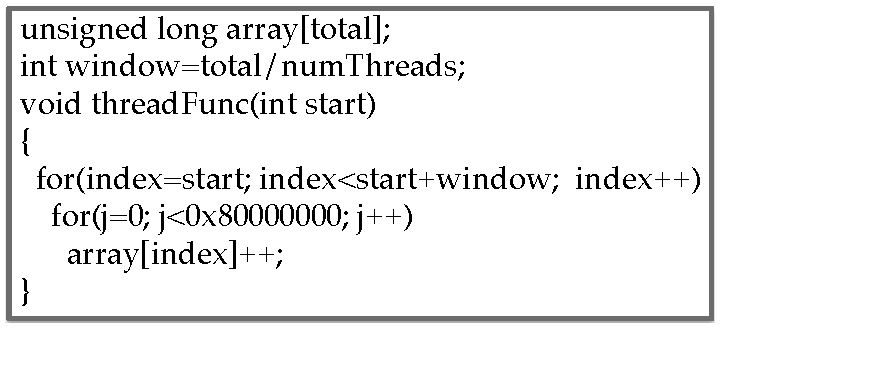
\includegraphics[width=2.8in]{figure/fscode}

}%
\hspace{30pt}
\subfigure[Performance Degradation]{%
   \label{fig:penaltyfig}
   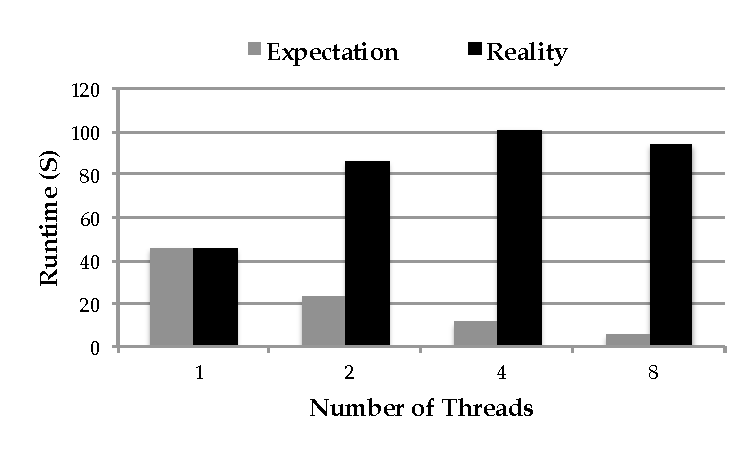
\includegraphics[width=2.4in]{figure/penalty}
}
\caption{
A false sharing example inside a multithreaded program (a) causes $13\times$ performance degradation (b) on a 8-core machine.
\label{fig:penalty}}
\end{figure*}

% Now we will talk about existing tools. 
False sharing problems like Figure~\ref{fig:penalty} are often invisible in the source code. Traditional profilers cannot be utilized to detect false sharing performance problems. For the example shown in Figure~\ref{fig:penalty}, ``gprof'' will show that  nearly 100\% time is spending on threadFunc~\cite{gprof}. This is the truth. But we cannot tell whether there is a false sharing problem inside or not.

Detecting false sharing problems needs special tools but existing false sharing detection have different types of problems: most cannot report precise information of false sharing, leaving much burden for programers for fixing~\cite{falseshare:binaryinstrumentation1,detect:ptu,detect:intel,falseshare:binaryinstrumentation2,DProf, qinzhao, OSdetection, mldetect, Wicaksono11detectingfalse, openmp}; some introduce too much performance overhead, making them impractical to be utilized in deployment environment~\cite{falseshare:binaryinstrumentation1,falseshare:binaryinstrumentation2,falseshare:simulator, Predator}; some require special OS support ~\cite{OSdetection} or only work on a special type of applications~\cite{sheriff}.

\vspace{0.2in}

\cheetah{} avoids all of these existing problems and has the following nice properties.

\begin{itemize} 
\item \cheetah{} can report precise information about false sharing problems. Like those precise tools, e.g. Sheriff~\cite{sheriff} and Predator~\cite{Predator}, it will pinpoint the lines of code where those variables or objects have false sharing problems. More than that, \cheetah{} can further pinpoint statements exercising false sharing problems, which can help programmers to fix found problems. 

\item Leveraging on hardware performance counters, \cheetah{} significantly reduces the performance overhead of detection, with only 5\% average performance overhead and 10\% maximum overhead. The performance overhead is similar to recent work~\cite{mldetect, openmp}, but with more precise information and more effectiveness.
  
\item Different with all existing tools, \Cheetah{} can predict the performance improvement after fixes based on latency information provided by performance counters. Based on that, \Cheetah{} can avoid reporting those insignificant problems, further reducing programmers burden. 

\end{itemize}





